\section*{Misure ed elaborazione dati}
\everymath{\displaystyle}
\begin{table}[h!]
    
    \hspace{5mm} 
    \begin{tabular}{|c|c|c|}
        \hline
        $i$ & $d_i$ (diametro) & $c_i$ (circonferenza)\\
        \hline

        1  & $37.0 \;mm \pm 0.5 \;mm$ & $116 \;mm \pm 1 \;mm$\\ 
        2  & $54.0 \;mm \pm 0.5 \;mm$ & $171 \;mm \pm 1 \;mm$\\ 
        3  & $61.0 \;mm \pm 0.5 \;mm$ & $192 \;mm \pm 1 \;mm$\\ 
        4  & $70.5 \;mm \pm 0.5 \;mm$ & $218 \;mm \pm 1 \;mm$\\ 
        5  & $85.5 \;mm \pm 0.5 \;mm$ & $271 \;mm \pm 1 \;mm$\\ 
        6  & $89.5 \;mm \pm 0.5 \;mm$ & $279 \;mm \pm 1 \;mm$\\ 
        7  & $104.5 \;mm \pm 0.5 \;mm$ & $325 \;mm \pm 1 \;mm$\\ 
        8  & $134.0 \;mm \pm 0.5 \;mm$ & $408 \;mm \pm 1 \;mm$\\ 
        9  & $149.5 \;mm \pm 0.5 \;mm$ & $466 \;mm \pm 1 \;mm$\\ 
        10 & $151.0 \;mm \pm 0.5 \;mm$ & $476 \;mm \pm 1 \;mm$\\ 
        11 & $167.5 \;mm \pm 0.5 \;mm$ & $531 \;mm \pm 1 \;mm$\\ 
        12 & $198.5 \;mm \pm 0.5 \;mm$ & $625 \;mm \pm 1 \;mm$\\ 
        13 & $211.0 \;mm \pm 0.5 \;mm$ & $660 \;mm \pm 1 \;mm$\\ 
        14 & $220.0 \;mm \pm 0.5 \;mm$ & $688 \;mm \pm 1 \;mm$\\ 
        15 & $293.5 \;mm \pm 0.5 \;mm$ & $911 \;mm \pm 1 \;mm$\\ 


        \hline
    \end{tabular}
    \caption{Misure rilevate}
    \label{tabellaDati}
\end{table}

\nls
\begin{plt}[h!]
    \hspace{5mm}
    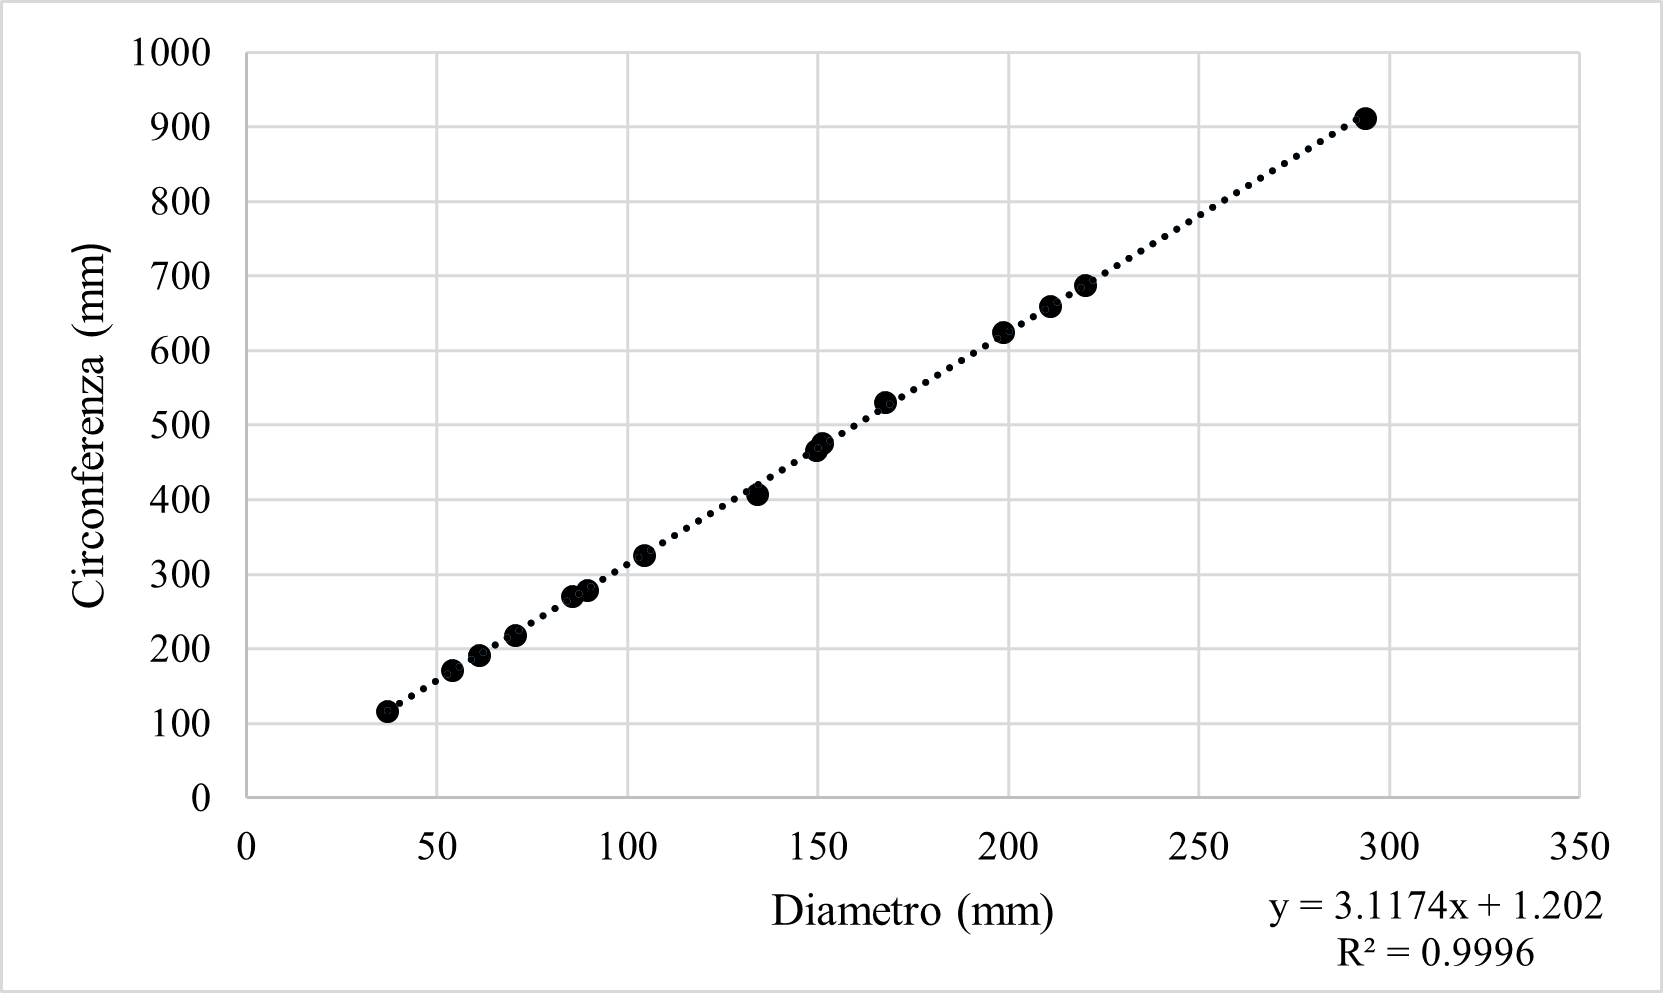
\includegraphics[width=10cm]{plots/plt1.png}
    \caption{Relazione tra circonferenza e diametro}
    \label{plt1}
\end{plt}
\newpage
Detto $n = 15$ il numero di misurazioni effettuate si ha che:\\ \\ 
$\overline{\pi} = \frac{1}{n}\sum_{i=1}^{n} \frac{c_i}{d_i} = 3.128$\\ 
\snls
Dati $\qq \overline{c} = \frac{1}{n} \sum_{i = 1}^{n} c_i = 422\;mm \qqq  \overline{d} = \frac{1}{n} \sum_{i = 1}^{n} d_i = 135.1\;mm$\\ 
si considera la funzione $f(c,d) = \frac{c}{d}$; dunque, tramite analisi della propagazione dell'errore di misura, si ottiene: \\ \\ 
$\Delta \pi = \sqrt{\left(\left|\frac{\partial f(c,d)}{\partial c} \right|_{\overline{c}, \overline{d}} \Delta c \right)^2 +
\left(\left|\frac{\partial f(c,d)}{\partial d} \right|_{\overline{c}, \overline{d}} \Delta d \right)^2} = 
\sqrt{\left(\left|\frac{\partial \frac{c}{d}}{\partial c} \right|_{\overline{c}, \overline{d}} \Delta c \right)^2 +
\left(\left|\frac{\partial \frac{c}{d}}{\partial d} \right|_{\overline{c}, \overline{d}} \Delta d \right)^2} \\ 
= \sqrt{\left(\frac{1}{\overline{d}} \Delta c \right)^2 +
\left(-\frac{\overline{c}}{\left(\overline{d}\right)^2} \Delta d \right)^2} = 0.014$\\ 
\snls 
Si riportano anche i valori di semidispersione, deviazione standard e coefficiente di correlazione lineare quadratico:\\ \\ 
$\frac{\pi_{max}- \pi_{min}}{2} = 0.06$\\\\
$\sigma_{\pi} = \sqrt{\frac{1}{n}\sum_{i=1}^{n}(\overline{\pi}-\pi_i)^2} = 0.03$\\\\
$R^2 = 0.9996$
